\section{Especificação de Requisitos}

\subsection{Descrição de Casos de Uso}

\subsubsection{Cadastrar Paciente}
\begin{table}[H]
  \centering
  \begin{tabular}{|p{4cm}|p{11cm}|}
    \hline
    \textbf{Identificador} & UC01 \\ \hline
    \textbf{Importância} & Essencial \\ \hline
    \textbf{Sumário} & Permite criar um novo registro no sistema representando um indivíduo que receberá cuidados na clínica. \\ \hline
    \textbf{Atores} & Recepcionista \\ \hline
    \textbf{Pré-condições} & O ator deve estar autenticado e o paciente deve fornecer dados válidos de identificação e contato. \\ \hline
    \textbf{Fluxo principal} & 
    1. O ator acessa a tela de cadastro.\newline
    2. O sistema exibe o formulário de cadastro.\newline
    3. O ator preenche os dados demográficos e contatos.\newline
    4. O ator solicita salvar os dados.\newline
    5. O sistema valida as informações.\newline
    6. O sistema registra o cadastro e vincula um identificador único.\newline
    7. O sistema informa o sucesso da operação. \\ \hline
    \textbf{Fluxos de exceção} & 
    - FE1: Se os dados forem inválidos, o sistema informa os campos com inconsistência e volta para o passo 3.\newline
    - FE2: O CPF já está vinculado, o sistema informa a duplicidade e oferece atalho para o perfil. \\ \hline
    \textbf{Pós-condição} & Um novo registro de paciente é salvo no banco de dados. O paciente fica disponível para agendamentos. \\ \hline
  \end{tabular}
\end{table}

\subsubsection{Agendar Consulta}
\begin{table}[H]
  \centering
  \begin{tabular}{|p{4cm}|p{11cm}|}
    \hline
    \textbf{Identificador} & UC02 \\ \hline
    \textbf{Importância} & Essencial \\ \hline
    \textbf{Sumário} & Permite definir uma reserva de tempo entre o paciente, o profissional e a clínica. \\ \hline
    \textbf{Atores} & Recepcionista, Paciente \\ \hline
    \textbf{Pré-condições} & O paciente deve existir no sistema e o profissional deve ter horários de agenda disponíveis. \\ \hline
    \textbf{Fluxo principal} & 
    1. O ator seleciona um Paciente na base de dados.\newline
    2. O ator escolhe a opção ``Agendar Consulta''.\newline
    3. O ator escolhe a especialidade e o profissional de Saúde.\newline
    4. O sistema consulta a Grade de Agenda (Schedule).\newline
    5. O sistema lista os horários disponíveis (Slot).\newline
    6. O ator seleciona data e horário.\newline
    7. O ator confirma o agendamento.\newline
    8. O sistema atualiza o status da agenda e salva a consulta.\newline
    9. O sistema agenda o disparo de um lembrete automático. \\ \hline
    \textbf{Fluxos de exceção} & 
    - FE1: O ator busca uma consulta existente e altera apenas o Slot de tempo para reagendamento. O sistema cancela o slot anterior e ocupa o novo. \\ \hline
    \textbf{Pós-condição} & Uma consulta é gerada com status ``agendado'' e um lembrete é engatilhado. \\ \hline
  \end{tabular}
\end{table}

\subsubsection{Registrar Atendimento Básico}
\begin{table}[H]
  \centering
  \begin{tabular}{|p{4cm}|p{11cm}|}
    \hline
    \textbf{Identificador} & UC03 \\ \hline
    \textbf{Importância} & Essencial \\ \hline
    \textbf{Sumário} & Permite que o profissional registre que a consulta ocorreu, suas observações e finalização. \\ \hline
    \textbf{Atores} & Profissional de saúde \\ \hline
    \textbf{Pré-condições} & O ator deve estar autenticado. Uma consulta deve existir para o dia corrente com status ``aguardando atendimento''. \\ \hline
    \textbf{Fluxo principal} & 
    1. O ator visualiza a fila de pacientes do dia.\newline
    2. O ator seleciona o paciente em espera e inicia o atendimento.\newline
    3. O sistema vincula o status do agendamento para ``em andamento''.\newline
    4. O ator documenta o motivo da visita, o histórico atual e aferições básicas.\newline
    5. O ator adiciona possíveis condições ou diagnósticos.\newline
    6. O ator encerra o atendimento.\newline
    7. O sistema altera o status do encontro para ``finalizado'' e salva no histórico geral. \\ \hline
    \textbf{Pós-condição} & O encontro clínico é salvo com status ``finalizado''. Possíveis problemas ou anotações ficam registrados no histórico do paciente. \\ \hline
  \end{tabular}
\end{table}

\subsection{Diagrama Casos de Uso}
Considerando os usuários do sistema, que foram identificados como os atores, e os requisitos documentados anteriormente, foi possível definir o diagrama de caso de uso (Figura~\ref{fig:diagrama_uc}), ilustrando as diversas interações que os usuários terão com o sistema.

\begin{figure}[H]
  \centering
  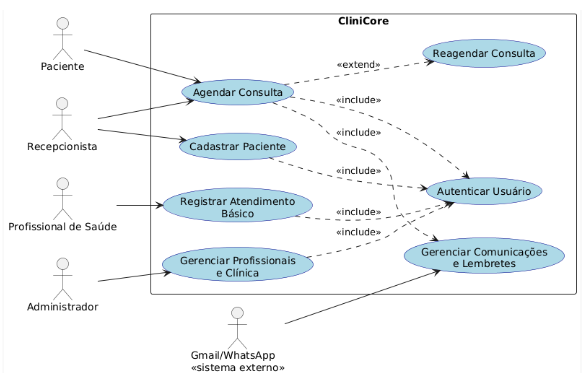
\includegraphics[width=0.9\textwidth]{images/diagrama-casos-de-uso.png}
  \caption{Diagrama de Casos de Uso do CliniCore.}
  \label{fig:diagrama_uc}
\end{figure}